% --------------------------------------------------------------
\begin{frame}[fragile]
  \frametitle{Storage Facility}
Two storage facilities were needed. One would conduct spent fuel cooling from
the LWRs and the other would do the same for the SFRs. 
\begin{figure}[htbp!]
\begin{center}
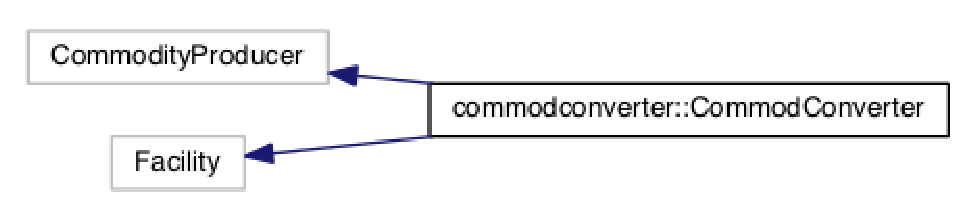
\includegraphics[width=0.8\textwidth]{cc_inherit}
\end{center}
\caption{Utilizes interfaces defined in Cyclus.}
\label{fig:cc_inherit}
\end{figure}
\end{frame}
% --------------------------------------------------------------
\begin{frame}[fragile]
  \frametitle{Archetype Definition}
Only one archetype is needed for this:  a simple representation of timed commodity transformation. 
 I called it CommodityConverter, and it accepts the following configuration variables:
\begin{itemize}
\item incoming commodity
\item outgoing commodity 
\item maximum capacity
\item delay time
\end{itemize}
\end{frame}
% --------------------------------------------------------------
\begin{frame}[fragile]
  \frametitle{Behavior}
After receiving a resource
(e.g., a material), this facility waits for a user-defined time period. Once
that time period has passed, the resource is offered to the resource exchange
system as a new commodity type. 
\end{frame}
% --------------------------------------------------------------
\begin{frame}[fragile]
  \frametitle{Code To Code Input Snippet}
\begin{lstlisting}
  <facility>
    <name>LWRWetStorage</name>
    <lifetime>1200</lifetime>
    <config>
      <CommodConverter>
        <in_commod>lwr_unf</in_commod>
        <in_recipe>lwr_unf_recipe</in_recipe>
        <out_commod>lwr_unf_cool</out_commod>
        <out_recipe>lwr_unf_recipe</out_recipe>
        <process_time>48</process_time>
      </CommodConverter>
    </config>
  </facility>
\end{lstlisting}
\end{frame}
